\documentclass{article}
\usepackage{listings}
\usepackage{graphicx}
\usepackage[slovene]{babel}
\usepackage{color}
\usepackage{amsmath}
\usepackage[usenames,dvipsnames]{xcolor}
\usepackage[hidelinks]{hyperref}
\usepackage{subcaption}
\usepackage{float}
\usepackage{rotating} 
\usepackage{hyperref}
\usepackage{caption}
\graphicspath{{./images/}}

\setlength{\parindent}{0pt}

\newcommand{\MAD}{\mathrm{MAD}}


\begin{document}

\title{Matematično-fizikalni praktikum \\[3mm] \large Naloga 3}
\author{Luka Papež}
\date{6.\ november 2024}

\begin{center}
    
\includegraphics[width=8cm]{logo-fmf.png}
\end{center}

{
    \let\newpage\relax
    \maketitle
}

\maketitle
\newpage
\section{Naloga}
Z diagonalizacijo poišči nekaj najnižjih lastnih
vrednosti in lastnih valovnih funkcij za moteno Hamiltonko
$H = H_0 + \lambda q^4$
ob vrednostih parametra $0\le\lambda\le 1$.  Rešujemo torej
matrični problem lastnih vrednosti
\begin{equation*}
  H | n \rangle = E_n | n \rangle \>.
\end{equation*}
Nove (popravljene) valovne funkcije $| n\rangle$ so seveda
linearna kombinacija starih (nemotenih) valovnih funkcij $| n^0\rangle$.
Matrike velikosti do $N=3$ ali $N=4$ lahko za silo diagonaliziramo peš;
za diagonalizacijo pri večjih $N$ uporabi enega ali več numeričnih postopkov,
na primer rutine {\tt tred2} in {\tt tqli}
iz zbirke Numerical Recipes ali iz kakega drugega vira (npr Python). Vsaj enega izmed
postopkov izvedi 'ročno' (sprogramiraj, uporabi izvorno kodo).  Preveri,
da v limiti $\lambda\to 0$ velja $E_n\to E_n^0$
(če ne velja, je verjetno nekaj narobe s programom).
Razišči, kako so rezultati odvisni od razsežnosti $N$ matrik
$H_0$ oziroma $q^4$.  Kakšna je konvergenca lastnih vrednosti
pri velikih $N$?

{\sl Dodatna naloga\/}: Poišči še nekaj najnižjih lastnih energij
in lastnih funkcij za problem v potencialu z dvema minimumoma
\begin{equation*}
H = {p^2\over 2} - 2q^2 + {q^4\over 10} \>.
\end{equation*}
\section{Uvod}
Enodimenzionalni linearni harmonski oscilator (delec mase $m$
s kinetično energijo $T(p)=p^2/2m$ v kvadratičnem potencialu
$V(q)=m\omega^2 q^2/2$) opišemo z brezdimenzijsko Hamiltonovo funkcijo
\begin{equation*}
  H_0 = {1\over 2} \left( p^2 + q^2 \right) \>,
\end{equation*}
tako da energijo merimo v enotah $\hbar\omega$, gibalne količine
v enotah $(\hbar m\omega)^{1/2}$ in dolžine v enotah $(\hbar/m\omega)^{1/2}$.
Lastna stanja $|n\rangle$ nemotenega Hamiltonovega operatorja $H_0$
poznamo iz osnovnega tečaja kvantne mehanike [Strnad III]:
v koordinatni reprezentaciji so lastne valovne funkcije
\begin{equation*}
  |n\rangle = (2^n n! \sqrt{\pi})^{-1/2} \mathrm{e}^{-q^2/2}\,  {\cal H}_n (q)\>,
\end{equation*}
kjer so ${\cal H}_n$ Hermitovi polinomi.
Lastne funkcije zadoščajo stacionarni Schr\"odingerjevi enačbi
\begin{equation*}
H_0 | n^0 \rangle = E_n^0 | n^0 \rangle
\end{equation*}
z nedegeneriranimi lastnimi energijami $E_n^0 = n + 1/2$
za $n=0,1,2,\ldots~$.  Matrika $\langle i | H_0 | j\rangle$
z $i,j=0,1,2,\ldots,N-1$ je očitno diagonalna, z vrednostmi
$\delta_{ij}(i + 1/2)$ po diagonali.  Nemoteni Hamiltonki
dodamo anharmonski člen
\begin{equation*}
H = H_0 + \lambda q^4 \>.
\end{equation*}
Kako se zaradi te motnje spremenijo lastne energije?
Iščemo torej matrične elemente $\langle i | H | j\rangle$
{\sl motenega\/} Hamiltonovega operatorja v bazi {\sl nemotenih\/}
valovnih funkcij $| n^0\rangle$, kar vemo iz perturbacijske
teorije v najnižjem redu.  Pri računu si pomagamo
s pričakovano vrednostjo prehodnega matričnega
elementa za posplošeno koordinato
$$
q_{ij} = \langle i | q | j \rangle
       = {1\over 2} \sqrt{i+j+1}\,\, \delta_{|i-j|,1} \>,
$$
ki, mimogrede, uteleša izbirno pravilo za električni dipolni
prehod med nivoji harmonskega oscilatorja.  V praktičnem računu
moramo seveda matriki $q_{ij}$ in $\langle i | H | j\rangle$
omejiti na neko končno razsežnost $N$.
\section{Računanje matrike}
Reševanje smo začeli z računanjem matrike, ki jo potem diagonaliziramo. Najprej konstruiramo matriko hamiltonke v anharmonskem potencialu 
$\langle i | H_0 + \lambda q^4 | j \rangle = \langle i | H_0 | j \rangle + \langle i | \lambda q^4 | j \rangle$.
Za izračun člena $\langle i | \lambda q^4 | j \rangle$ imamo tri možnosti. Lahko izračunamo $\langle i | q | j \rangle$, $\langle i | q^2 | j \rangle$ in jih potem matrično množimo, da pridemo do četrte potence. Zadnja možnost pa je direktno računanje $\langle i | q^4 | j \rangle$. Izračunamo jih po podanih formulah v navodilu:
\begin{equation*}
q_{ij} = \langle i | q | j \rangle
       = {1\over 2} \sqrt{i+j+1}\,\, \delta_{|i-j|,1} \>,
\end{equation*}
\begin{equation*}
\langle i|q^2|j\rangle
  = {1\over 2} \biggl[
    {\sqrt{j(j-1)}} \, \delta_{i,j-2}
  + {(2j+1)} \, \delta_{i,j}
  + {\sqrt{(j+1)(j+2)}} \, \delta_{i,j+2} \biggr]
\end{equation*}
\begin{eqnarray*}
\langle i|q^4|j\rangle
  = {1\over 2^4}\sqrt{2^i \, i!\over 2^{j} \, j! } \, \biggl[ \,
  &\,& \delta_{i,j+4} + 4\left(2j+3\right) \delta_{i,j+2}
                      + 12 \left(2j^2+2j+1\right) \, \delta_{i,j} \\[3pt]
  &+& 16j \left(2j^2-3j+1\right) \, \delta_{i,j-2}
     + 16j\left(j^3-6j^2+11j-6\right) \, \delta_{i,j-4} \biggr] \>,
\end{eqnarray*}
Najnatančnejše bo direktno računanje četrte potence. Poglejmo si še hitrost izračuna. Da poenostavimo računanje četrte potence in se znebimo `overflowov` implementiramo funkcijo, ki ulomek fakultet `pokrajša` in izračuna le številko, ki ostane. Z nekaj več truda pa bi lahko upoštevali tudi lastnosti delta funkcije in se fakultet popolnoma znebili.

\begin{figure}[H]
    \centering
    \begin{minipage}{0.49\textwidth}
        \centering
        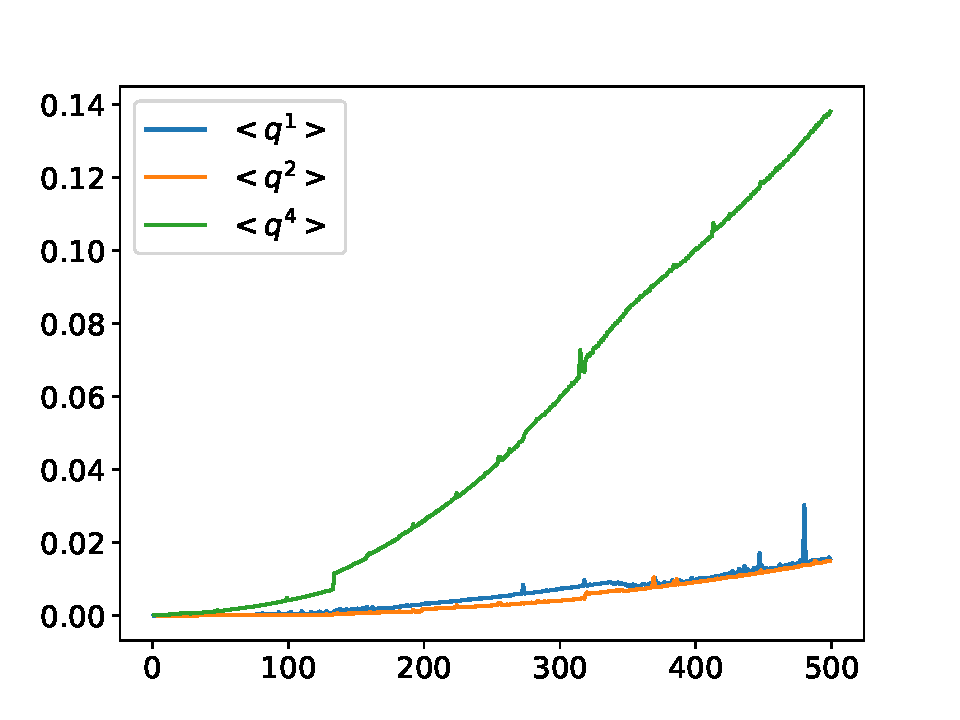
\includegraphics[width=\linewidth]{cpu.pdf}
        \caption{Računanje anharmonskega člena z `numpy`}
    \end{minipage}
    \hfill
    \begin{minipage}{0.49\textwidth}
        \centering
        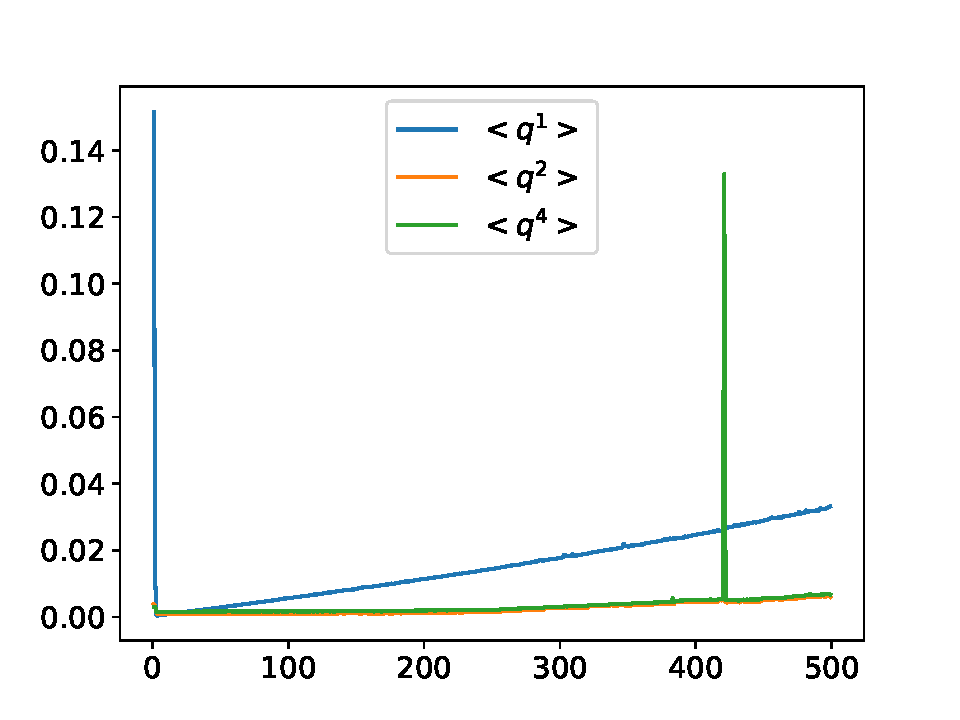
\includegraphics[width=\linewidth]{gpu.pdf}
        \caption{Računanje anharmonske člena s `cupy`}
    \end{minipage}
\end{figure}
Opazimo zanimive relacije. Pri računanju z numpy dobimo rahlo neintuitivne rezultate zaradi uporabe vektorizacije funkcije, ki je precej neučinkovita. To služi kot direktna primerjava s `cupyjevim elementwise`. Nenavadno je tudi, da so med prvo in drugo potenco tako majhne razlike, saj ima prva potenca q-ja dva matrična množenja v primerjavi z drugo, ki ima le eno. Osredotočimo se na računanje s `cupyjem`, kjer je `elementwise` precej bolj učinkovit, saj je `compilan`. Najprej si oglejmo špico, ki se pojavi na začetku grafa. Ta se je konsistentno pojavaljala čez vse poskuse in jo lahko enostavno pojasnimo z dejstvom, da ima `cupy` nek začetni čas, ki ga uporabi za inicializacijo. Tukaj prva potenca kar precej odstopa, saj ima dva matrična množenja. Pri tej potenci pa je tudi vredno omembe, da je hitrost primerljiva z izračunom s knjižnico `numpy`. Razlika pa je v hitrosti rasti, saj je ta pri `cupy` zgleda linearna v primeru `numpy` pa ne. Da bi to potrdili bi potrebovali izračunati še večje matrike in raziskati še druge možne vplive, kar pa presega obseg te naloge. Hitrost enega matričnega množenja in implementiranega `deljenje fakultet` pa je očitno tudi približno primerljiva. 
\newpage
\section{Diagonalizacija matrik}
\subsection{Lastne energije}
Da najdemo lastne energije anharmonskega oscilatorja moramo matriko naprej diagonalizirati. Poglejmo si najprej kako se obnašajo lastne energije oz. z drugimi besedami lastne vrednosti matrik anharmonske hamiltonke. 

\begin{figure}[H]
    \centering
    \begin{minipage}{0.49\textwidth}
        \centering
        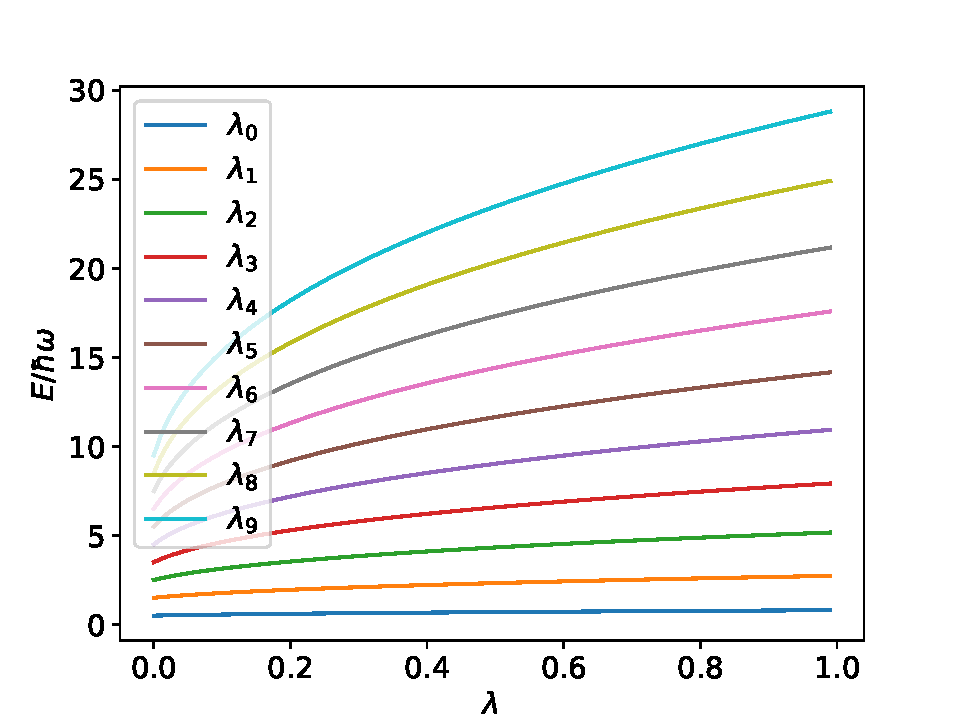
\includegraphics[width=\linewidth]{energyfromlambda.pdf}
        \caption{Prvih deset lastnih energij anharmonske hamiltonke v odvisnosti od $\lambda$}
    \end{minipage}
    \hfill
    \begin{minipage}{0.49\textwidth}
        \centering
        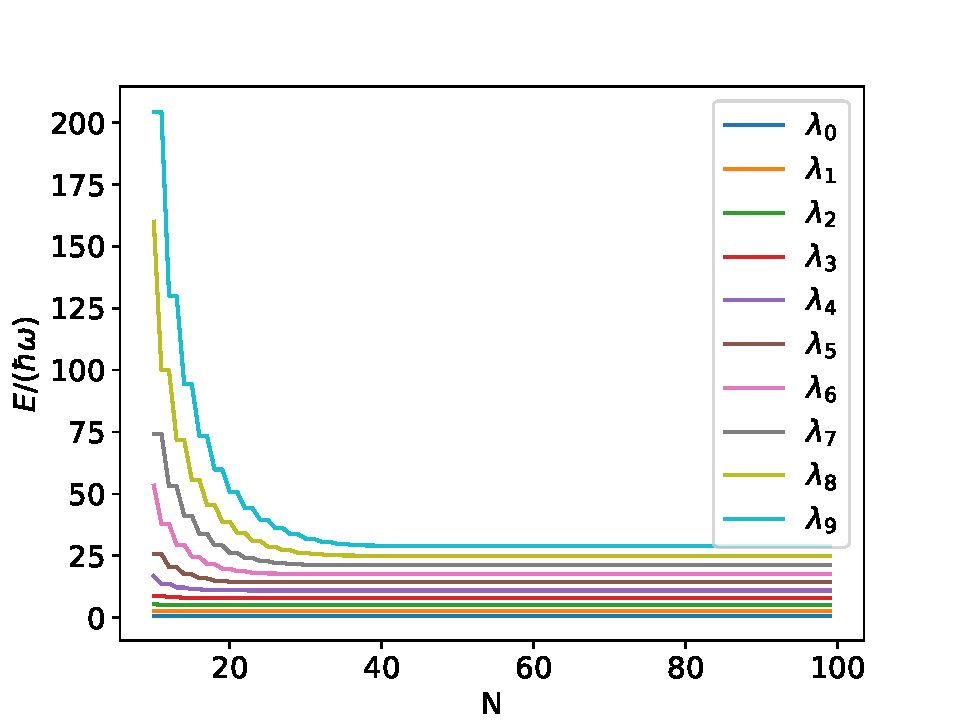
\includegraphics[width=\linewidth]{energyfromN.pdf}
        \caption{Prvih deset lastnih energij anharmonske hamiltonke v odvisnosti od velikosti matrike}
    \end{minipage}
\end{figure}
Pričakovano glede na potencial lastne energije naraščajo z lambdo. Na grafu odvisnosti od velikosti pa opazimo konvergenco k določeni vrednosti. To je logično, saj bi naše matrike v teoriji morale biti neskončne in zato z večjimi matrikami dobimo boljši približek. Pri nekaterih vrednostih pa se pojavijo rahle nezveznosti, ki imajo najverjetneje nek globji razlog. 

\subsection{Analiza hitrosti metod diagonalizacije}
Za diagonalizacijo smo uporabili pet različnih metod računanja, ki so vrnile precej različne rezultate čeprav so implementirane podobno. Metode lahko razdelimo v tri kategorije prva je implementacija Householderjeve metoda, ki je bila podana v navodilih. Druga pa je računanje z `numpy` (uporaba CPU) in tretja s `cupy` (uporaba GPU). V poskusu razjasnitve rezultatov pa smo uporabili tudi funkcionalnost njunih vgrajenih metod, ki omogočajo računanje lastnih vrednosti večih matrik hkrati. V obeh zadnjih kategorijah smo za izračun uporabljali funkcijo `.linalg.eigh`. 

\begin{figure}[H]
    \centering
	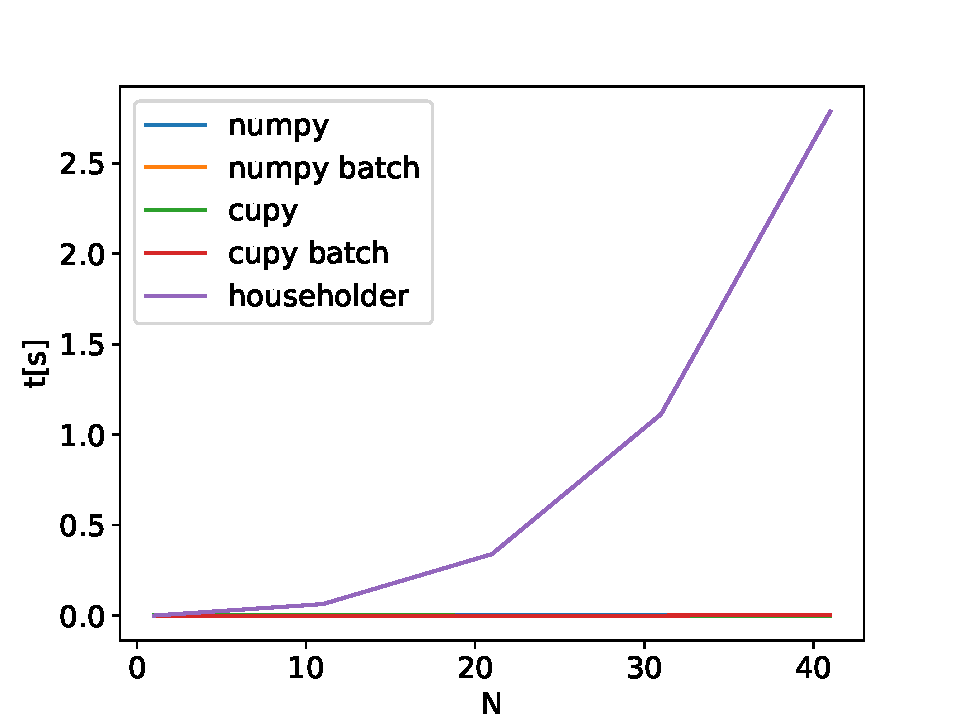
\includegraphics[width=0.6\textwidth]{householder.pdf}
    \caption{Primerjava hitrosti računanj lastnih vrednosti različnih metod}
\end{figure}

Iz grafa se jasno razbere, da je podana metoda prepočasna za dejansko uporabo, saj se že pri majhnih velikostih matrike čas poveča na nekaj sekund. Zato jo izločimo iz računanja in poglejmo obnašanje preostalih metod.

\begin{figure}[H]
    \centering
    \begin{minipage}{0.49\textwidth}
        \centering
        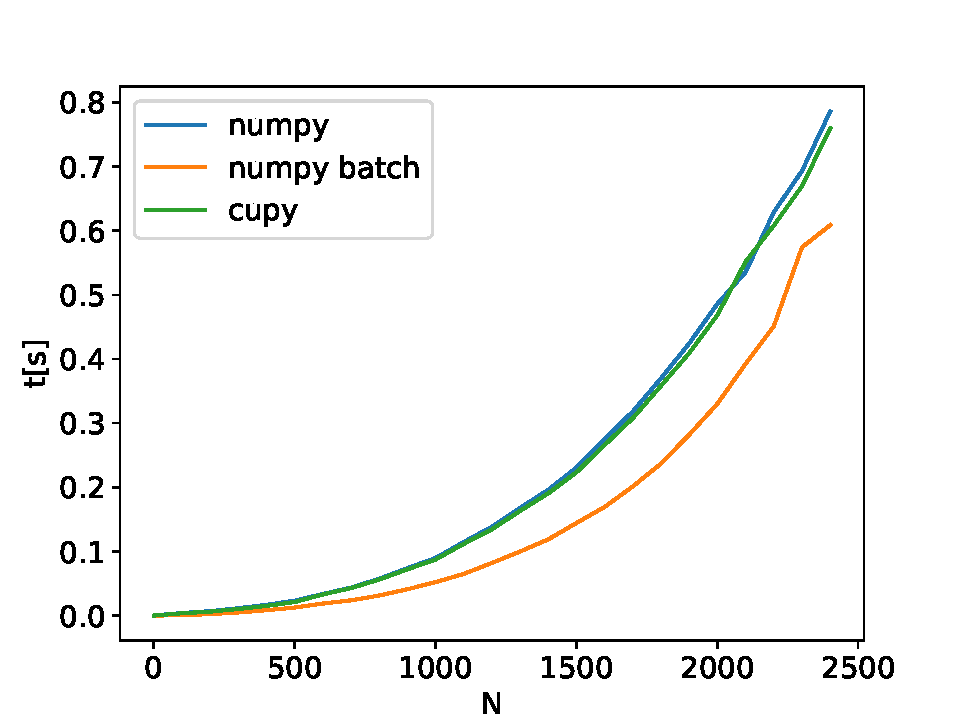
\includegraphics[width=\linewidth]{cuda.pdf}
    \end{minipage}
    \hfill
    \begin{minipage}{0.49\textwidth}
        \centering
        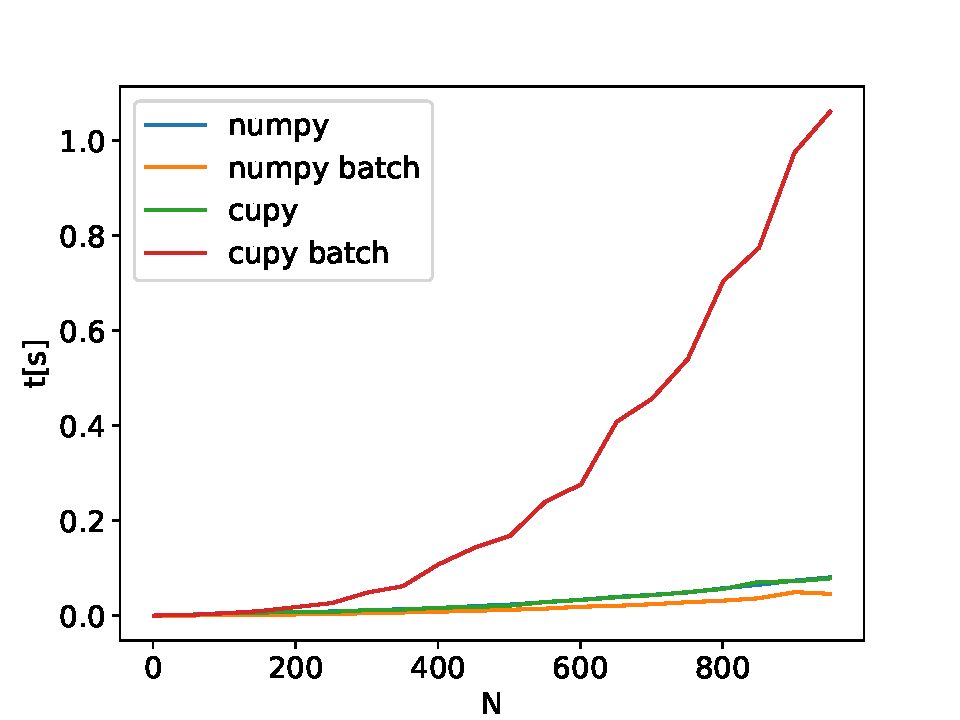
\includegraphics[width=\linewidth]{batch.pdf}
    \end{minipage}
	\caption{Primerjava hitrosti računanja lastnih vrednosti brez metode Householder}
\end{figure}
Majhna razlika med cupy in numpy je precej nepričakovana. Po nekaj raziskovanja ugotovimo, da je razlog za to dejstvo, da je komunikacija s CPU zelo hitra v primerjavi s komunikacijo z GPU. Sama operacija iskanja lastnih vrednosti pa je tudi hitra zato ne opazimo precejšnih razlik med njima. To nam, da misliti, da če prenesemo več matrik hkrati bo vpliv komunikacijskega časa precej manjši. Naša hipoteza se v primeru `numpy` potrdi, a zaradi že hitre komunikacije razlika ni bistvena. Pri `cupy` pa so rezultati popolnoma nasprotni našim pričakovanjem, čas se občutno poveča. Da izločimo morebitne posebnosti napišemo test računanja lastnih vrednosti na naključnih hermitskih matrikah in ga poženemo še na eni napravi. Rezultati se ponovijo. Morebitni razlogi zakaj je prišlo do takega odstopanja od ostalih metod so precej nejasni. Predvidevamo lahko, da je ponovno problem o prenosu podatkov in se ta upočasni ob prenosu večje količine podatkov, a to težko potrdimo.   

\subsection{Risanje lastnih funkcij}
Naši izračunani lastni vektorji anharmonske hamiltonke so v lastni bazi harmonskega oscilatorja. Zato lahko poznane rešitve lastnih funkcij harmonskega oscilatorja uporabimo za konstrukcijo lastnih funkcij anharmonskega oscilatorja. Dobljene lastne funkcije pa narišemo v potencialu okoli lastne energije kateri pripadajo. 


\begin{figure}[H]
    \centering
	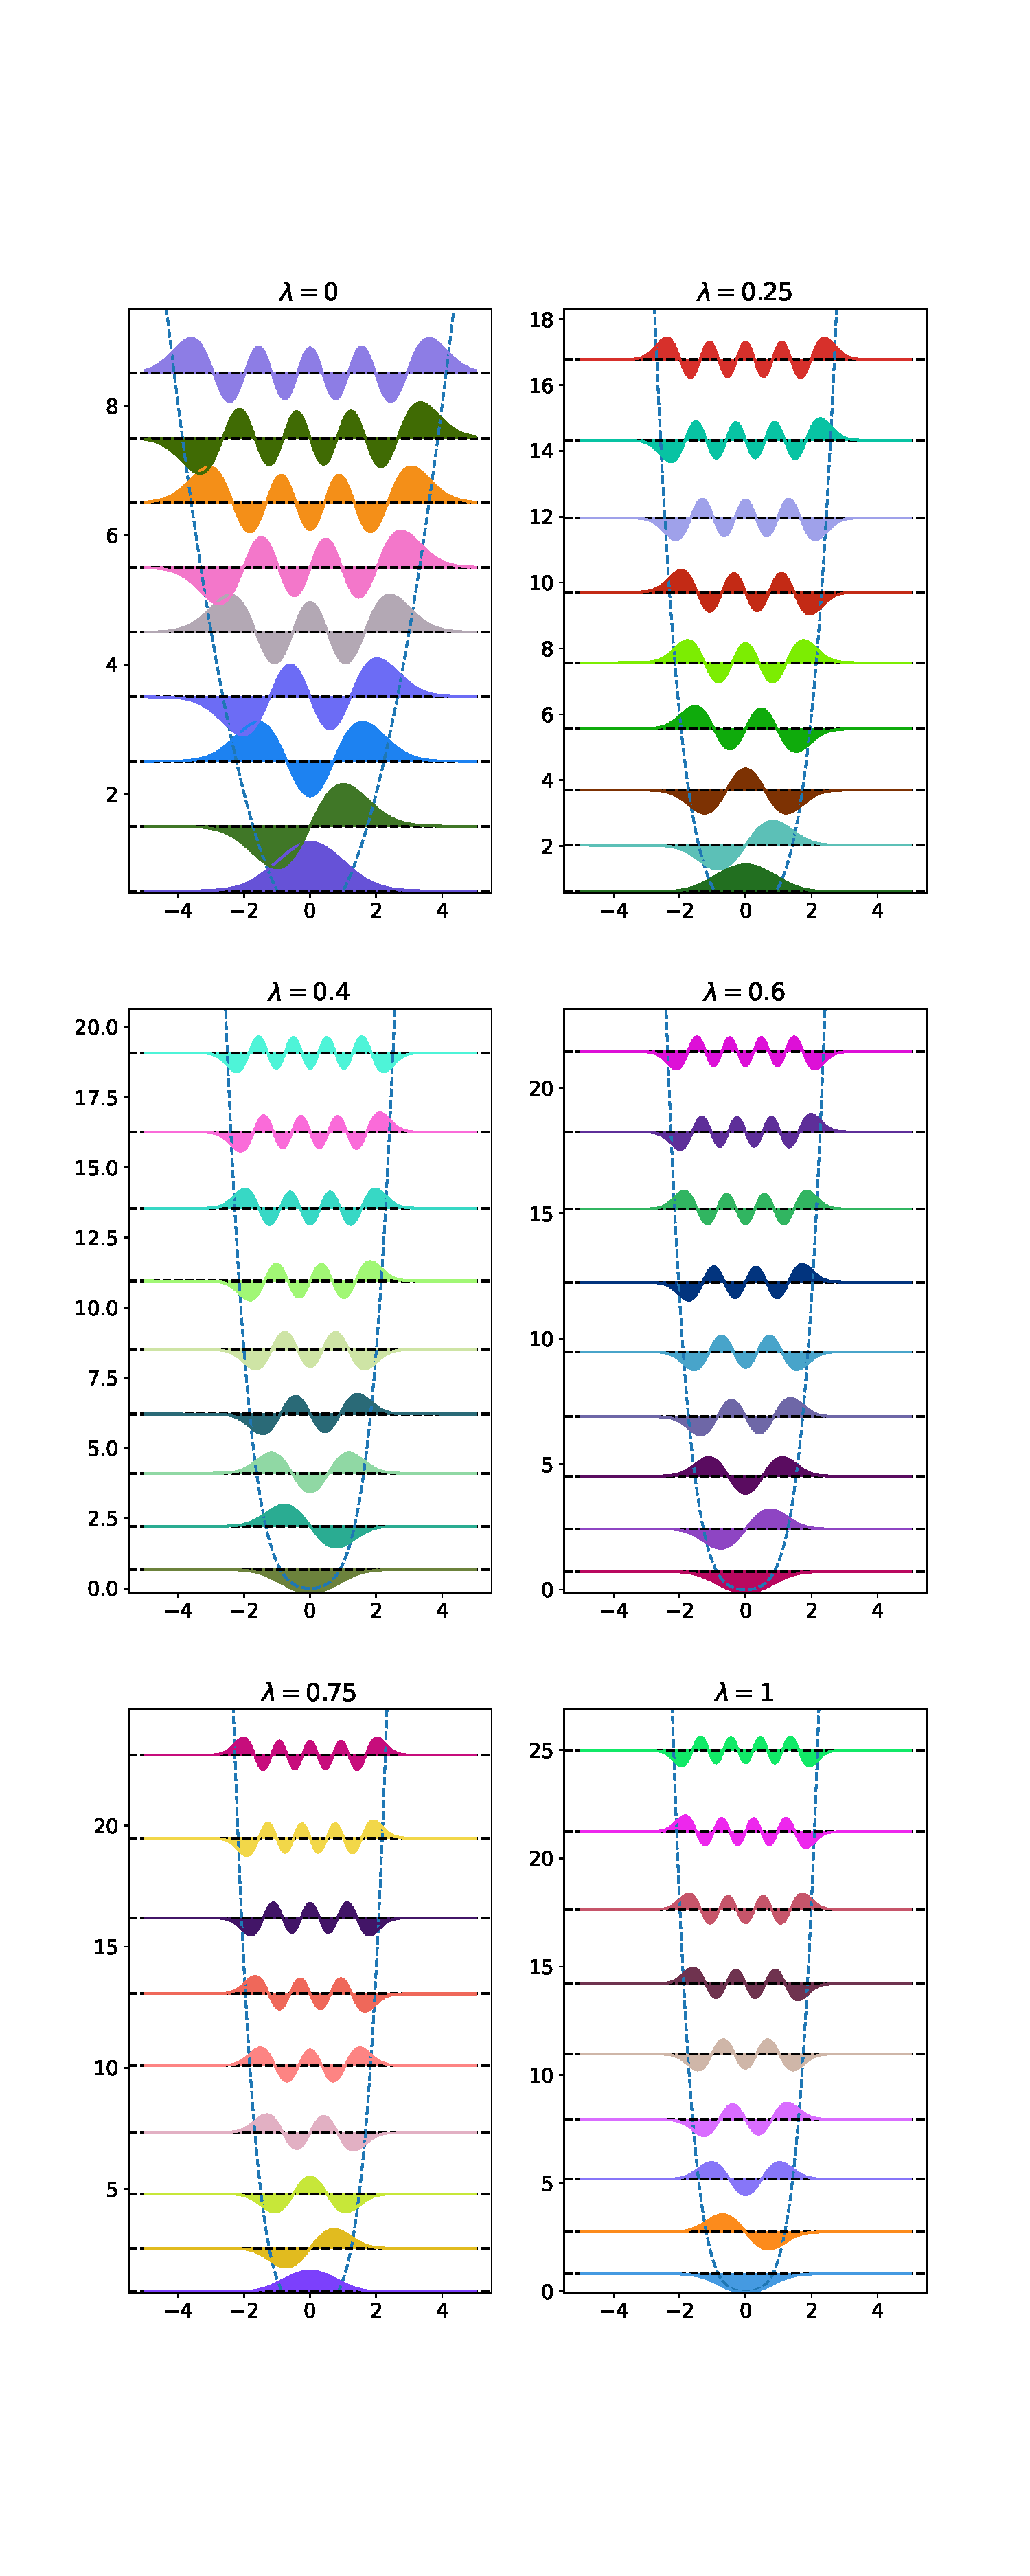
\includegraphics[width=0.7\textwidth]{eigenfunctions.pdf}
	\caption{Lastne funkcije anharmonskega oscilatorja na nivoju njihove lastne energije}
\end{figure}
Dobljeni grafi so konsistentni z našimi dosedanjimi opažanji in znanjem, kar nam potrdi pravilnost našega izračuna. Poglejmo si še dodatno nalogo iskanja lastnih energij in funkcij v potencialu z dvema minimuma. Rahlo preoblikujmo dano hamiltonko, da si olajšamo izračun matrike.
\begin{equation*}
	H = \frac{p^2}{2} - 2 q^2 + \frac{q^4}{10} = \frac{1}{2} (p^2 + q^2) - \frac{5}{2}q^2 + \frac{q^4}{10} = H_0 - \frac{5}{2}q^2 + \frac{q^4}{10}
\end{equation*}
\begin{figure}[H]
    \centering
	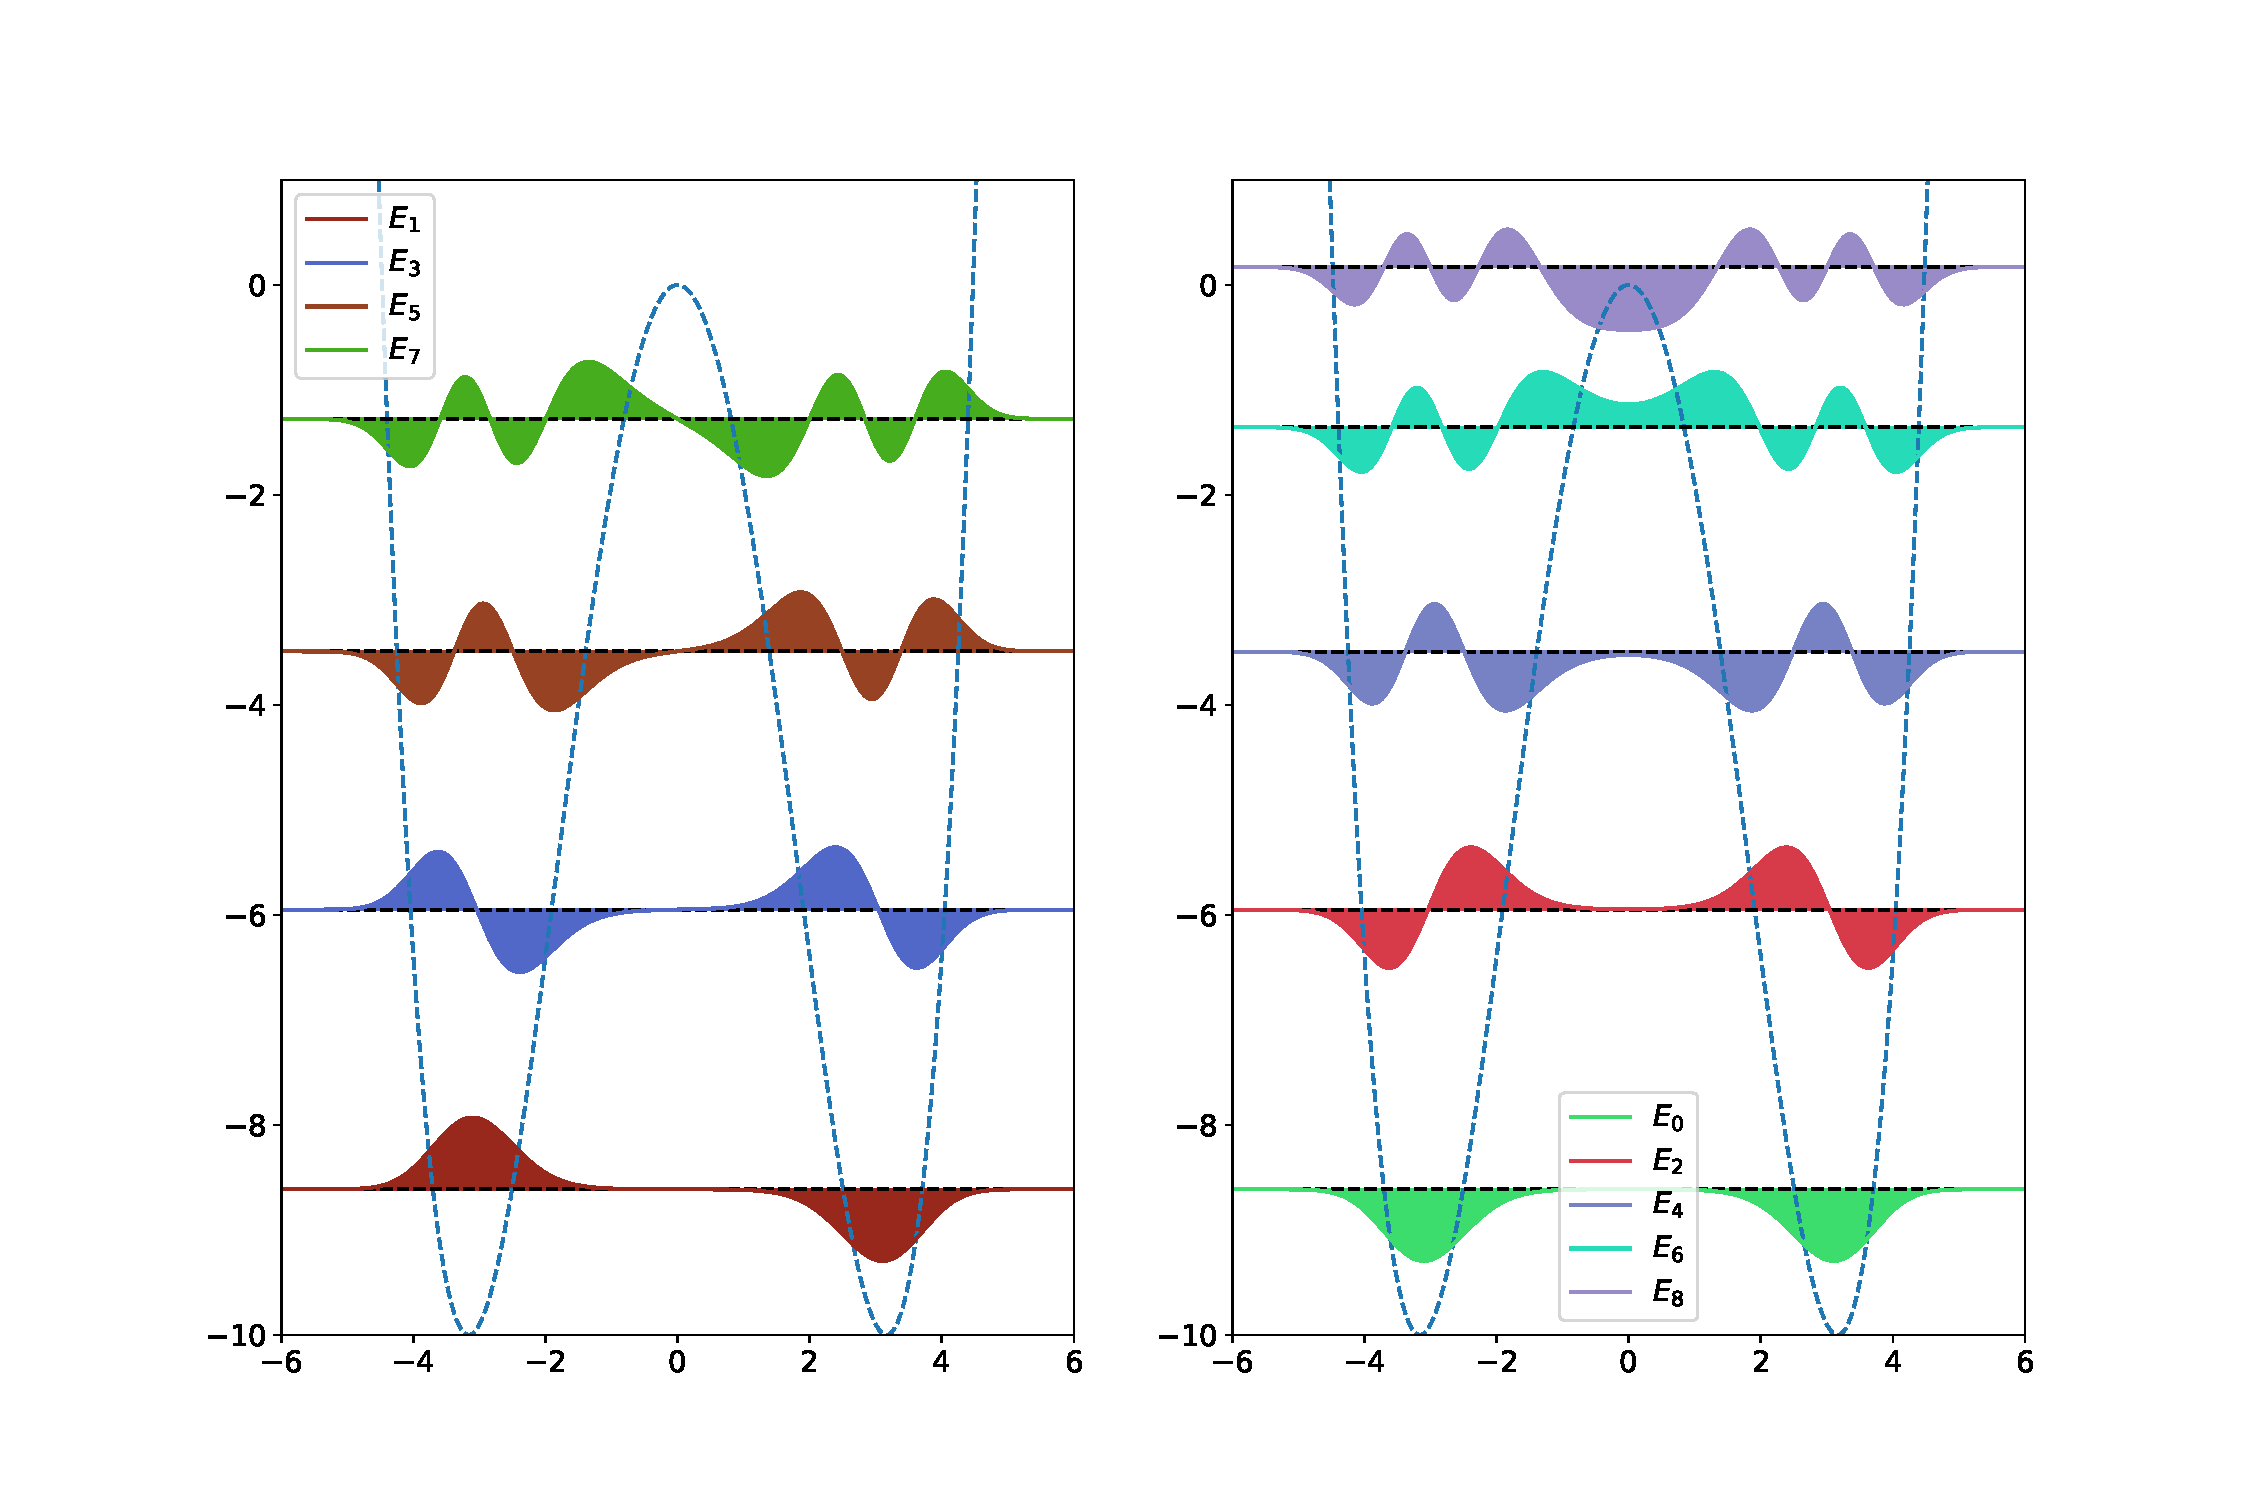
\includegraphics[width=0.7\textwidth]{extra.pdf}
	\caption{Lastne funkcije v potencialu $V=-2q^2 + \frac{q^4}{10}$} 
\end{figure}
Sodi in lihi pari funkcij so skoraj degenerirani, a imajo rahlo odstopanja. Za boljšo preglednost jih zato na grafih ločimo.
\section{Zaključek}
Raziskali smo problem računanja lastnih vrednosti in vektorjev s pomočjo različnih metod. Ob reševanju problema sem se spoznal z delovanjem knjižnice `cupy`. To se mi je zdela uporabna izkušnja, saj sem precej naučil o omejitvah uporabe GPU in načinih njegove uporabe.  
\end{document}
